%
% Copyright (c) 2021 Antonio Coín Castro
%
% This work is licensed under a
% Creative Commons Attribution-ShareAlike 4.0 International License.
%
% You should have received a copy of the license along with this
% work. If not, see <http://creativecommons.org/licenses/by-sa/4.0/>.
%

\RequirePackage{fix-cm}
\documentclass[10pt, professionalfonts]{beamer}

\usepackage{pifont}  % xmark, cmark
\newcommand{\cmark}{\ding{51}}%
\newcommand{\xmark}{\ding{55}}%

% OPCIONES DE BEAMER

\definecolor{Maroon}{cmyk}{0, 0.87, 0.88, 0.1}
\definecolor{teal}{rgb}{0.0, 0.45, 0.45}

\usetheme[block=fill, subsectionpage=progressbar, titleformat section=smallcaps]{metropolis}
\setbeamertemplate{frametitle continuation}[roman]
\setbeamertemplate{section in toc}[balls numbered]
\setbeamertemplate{subsection in toc}[subsections unnumbered]
%\setsansfont[BviejoFont={Fira Sans SemiBold}]{Fira Sans Book}  % Increase font weigth
\widowpenalties 1 10000
\raggedbottom

% COLORES
\setbeamercolor{palette primary}{bg=teal}
\setbeamercolor{progress bar}{use=Maroon, fg=Maroon}

% PAQUETES

\usepackage[style=apa]{biblatex}
\usepackage[utf8]{inputenc}
\usepackage[absolute,overlay]{textpos}
\usepackage[spanish, es-nodecimaldot]{babel}
\usepackage{microtype}
\usepackage{epigraph}
\usepackage{hyperref}
\usepackage{amssymb, amsmath, amsthm, amsfonts, amscd}
\usepackage{listings}

\DefineBibliographyStrings{spanish}{%
  andothers = {et\addabbrvspace al\adddot}
}

\addbibresource{bibliography.bib}

% FONTS
%\usefonttheme{professionalfonts}
%\usepackage{mathpazo}
%\usepackage{eulervm}

\definecolor{backg}{HTML}{F2F2F2} % Fondo
\definecolor{comments}{HTML}{a8a8a8} % Comentarios
\definecolor{keywords}{HTML}{08388c} % Palabras clave
\definecolor{strings}{HTML}{0489B1}  % Strings

\lstset{
language=scala,
basicstyle=\footnotesize\ttfamily,
breaklines=true,
keywordstyle=\color{keywords},
commentstyle=\color{comments},
stringstyle=\color{strings},
xleftmargin=.5cm,
tabsize=2,
% Acentos, ñ, ¿, ¡ (tex.stackexchange.com/questions/24528)
extendedchars=true
}

\hypersetup{
    colorlinks,
    citecolor=blue!50!black,
    linkcolor=black
}

% COMANDOS PERSONALIZADOS

\let\lmin\wedge
\let\lmax\vee
\newtheorem{prop}{Proposición}
\newtheorem{teorema}{Teorema}
\newtheorem{defi}{Definición}
\newcommand\ddfrac[2]{\frac{\displaystyle #1}{\displaystyle #2}}  % Fracción grande

% TÍTULO

\title{Resultados actualizados y otros algoritmos de comparación}
\providecommand{\subtitle}[1]{}
\subtitle{Regresión y clasificación funcional}
\date{\today \\}
\author{Antonio Coín}% \\ José R. Berrendero \\ Antonio Cuevas\\}
\institute{Universidad Autónoma de Madrid \\ \textit{Departamento de Matemáticas}}

\titlegraphic{
  \begin{textblock*}{2cm}(9.8cm,6.1cm)
    
\includegraphics[width=2cm]{img/logo-uam}
  \end{textblock*}
}
% DOCUMENTO

\begin{document}
\maketitle

\section{Partial Least Squares (PLS)}

\begin{frame}{PLS multivariante}

Se trata de un \textit{método supervisado}. Descomponemos
\[
X = TP^T, \quad Y = UQ^T
\]
de forma que se maximice la \textbf{covarianza} entre X e Y (algoritmo PLS1).

Una vez aprendida la transformación, podemos realizar regresión lineal de dos maneras:

\begin{itemize}
  \item Utilizando las transformaciones de X e Y para expresar $Y=X\beta$ a partir de ellas (PLS Regression).
  \item Transformando los datos $X_i\leftrightsquigarrow T_i$ y aplicando \textbf{cualquier} método de regresión multivariante sobre el conjunto $(\{T_i, Y_i\})$, donde ahora $T_i$ son datos de dimensión posiblemente menor (reducción de dimensionalidad).
\end{itemize}
\end{frame}

\begin{frame}{PLS Funcional}
  El algoritmo PLS multivariante se puede aplicar directamente a los datos funcionales (discretizados) para reducir la dimensión de los mismos. Sin embargo, existe una extensión puramente funcional \parencite{preda2002pls} que se basa en el siguiente problema de optimización:
  \[
  \max_{w, c} \ \operatorname{Cov}^2\left( \int_{\mathcal T} X(t)w(t)\, dt, cY\right).
  \]

Se define la primera componente principal PLS como la variable aleatoria
\[
t_1 = \int_{\mathcal T} X(t)w(t)\, dt,
\]

y se sigue un proceso iterativo análogo al caso finito-dimensional para encontrar el resto de componentes.

\end{frame}

\begin{frame}{Implementación PLS funcional I}

    {\color{Maroon}\textbf{Caso I (extensión multivariante)}:} utilizar un desarrollo en base.

    \vspace{1em}

    Supongamos que tenemos los datos desarrollados en una base $X_i(t)=\sum_j \alpha_{ij} \phi_j(t)$. En \textcite{aguilera2010using} se demuestra que la regresión PLS funcional de $Y$ sobre $X$ es equivalente a la regresión PLS multivariante de $Y$ sobre $A\Phi^{1/2}$, donde $A=(\alpha_{ij})$ es la matriz de coeficientes y $\Phi$ es la matriz de Gram de los elementos de la base.

    \textbf{Implementación:} casi inmediata usando librerías de regresión PLS multivariante.

\end{frame}

\begin{frame}{Implementación PLS funcional II}

  {\color{Maroon}\textbf{Caso II (puramente funcional)}:} obtener una \textbf{base de componentes PLS} directamente a partir de los datos.
  \vspace{1em}

  Se trata del algoritmo APLS \parencite{delaigle2012methodology}. Presenta un enfoque alternativo donde se construyen secuencialmente $h$ funciones ortonormales $\{\phi_p(t)\}_{p=1,\dots,h}$ para maximizar
  \[
  \operatorname{Cov}\left(Y - g_{p-1}(X), \int_{\mathcal T}X\phi_p\right),
  \]
  donde $g_p(x) = \sum_{j=1}^p \beta_j \int_{\mathcal T}x\phi_j$. Los valores óptimos de $\beta$ se encuentran empíricamente por mínimos cuadrados. Finalmente, predecimos con $g_h$.

  \textbf{Implementación:} es necesario aproximar integrales numéricamente y utilizar el algoritmo de Gram-Schmidt.
\end{frame}

\section{LDA y regresión lineal}

%[ver referencias en http://eric.univ-lyon2.fr/~ricco/tanagra/fichiers/en_Tanagra_LDA_and_Regression.pdf]

% \textit{This shows that the solution to the least squares problem is in the same direction as the solution of Fishers discriminant, although it will have a different length. But as we already noticed, we are only interested in the direction of w, not its length and hence the solutions are identical} (sin tener en cuenta el bias).


\begin{frame}{LDA}

El algoritmo de \textit{Linear Discriminant Analysis} para el caso de clasificación binaria es equivalente{\footnote{Salvo por el término independiente; ver \textcite{hart2000pattern, mika2003kernel, gareth2013introduction}.}} a la regresión lineal por mínimos cuadrados (usando un umbral de decisión). Lo mismo ocurre con sus respectivas extensiones al caso funcional, que en el caso de LDA persigue encontrar combinaciones lineales (en $L^2$) $\Phi(X)$ de los predictores para maximizar
\[
\frac{\operatorname{Var}(\mathbb E[\Phi(X)\mid Y ])}{\operatorname{Var}(\Phi(X))},
\]

y en el caso de la regresión lineal trata de modelar la relación $Y=\Phi(X)+\varepsilon$. La regla de clasificación resultante para un umbral $t$ es $g(x) = \mathbb I(\Phi(x) > t)$. Este umbral de decisión se fija \textit{de facto} a la media ponderada de las respuestas codificadas $Y=\{y_0, y_1\}$:
\[
t = p_0y_0 + p_1y_1, \quad \text{con } p_i = n_i/n.
\]

\end{frame}

\begin{frame}{Regresión PLS para clasificación}

En el caso funcional, el uso de regresión lineal para clasificación presenta algunos problemas \parencite[y referencias contenidas]{preda2005pls}. En este mismo artículo se propone usar la regresión PLS para aproximar la función discriminante.
\vspace{1em}

\textbf{Algoritmo:}
\begin{enumerate}
  \item Recodificar las etiquetas $0 \leftrightsquigarrow -\sqrt{p_1/p_0}$ y $1 \leftrightsquigarrow \sqrt{p_0/p_1}$.
  \item Realizar regresión PLS de $Y$ sobre $X$ para obtener $\Phi_{PLS}(X) = \int_{\mathcal T}X(t)\beta_{PLS}(t)\, dt$.
  \item Clasificar en la clase 0 si $\mathbb I(\Phi_{PLS}(x) < 0)$.
\end{enumerate}
\end{frame}

\section{Resultados}

\begin{frame}{Nota sobre las implementaciones}

En una búsqueda rápida no se encontraron ninguno de los métodos funcionales comentados anteriormente implementados directamente en Python. Se ha hecho una implementación vectorizada (intentando maximizar la eficiencia) y al estilo del paquete \textit{scikit-fda}, lo que permitiría fácilmente su integración en el mismo.

\end{frame}

\subsection{Regresión lineal}

\begin{frame}{Resultados RKHS kernel fBM}
  \begin{figure}
    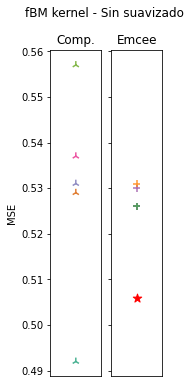
\includegraphics[width=0.3\textwidth]{img/results-new/reg_rkhs_fbm_none}\hfill
    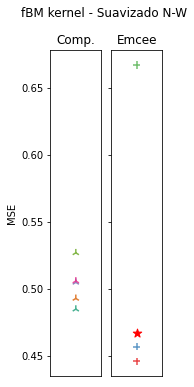
\includegraphics[width=0.3\textwidth]{img/results-new/reg_rkhs_fbm_nw}\hfill
    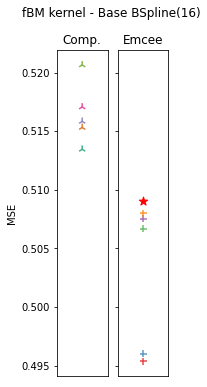
\includegraphics[width=0.32\textwidth]{img/results-new/reg_rkhs_fbm_basis}
    \caption{MSE de los mejores estimadores en cada caso bajo el modelo subyacente RKHS con kernel Browniano fraccional.}
  \end{figure}
\end{frame}

\begin{frame}{Resultados RKHS kernel O-U}
  \begin{figure}
    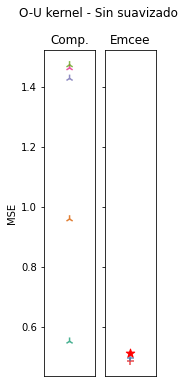
\includegraphics[width=0.3\textwidth]{img/results-new/reg_rkhs_ou_none}\hfill
    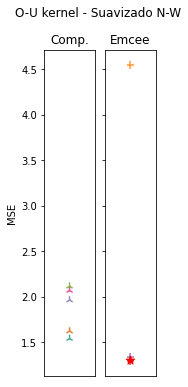
\includegraphics[width=0.3\textwidth]{img/results-new/reg_rkhs_ou_nw}\hfill
    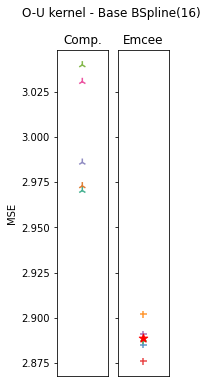
\includegraphics[width=0.33\textwidth]{img/results-new/reg_rkhs_ou_basis}
    \caption{MSE de los mejores estimadores en cada caso bajo el modelo subyacente RKHS con kernel de Ornstein-Uhlenbeck.}
  \end{figure}
\end{frame}

\begin{frame}{Resultados RKHS kernel RBF}
  \begin{figure}
    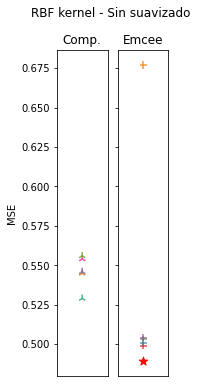
\includegraphics[width=0.31\textwidth]{img/results-new/reg_rkhs_rbf_none}\hfill
    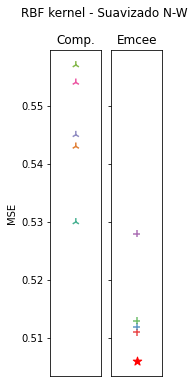
\includegraphics[width=0.3\textwidth]{img/results-new/reg_rkhs_rbf_nw}\hfill
    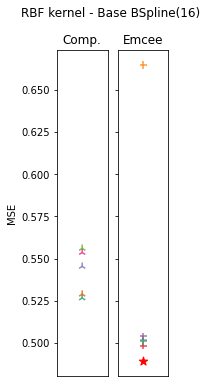
\includegraphics[width=0.32\textwidth]{img/results-new/reg_rkhs_rbf_basis}
    \caption{MSE de los mejores estimadores en cada caso bajo el modelo subyacente RKHS con kernel RBF.}
  \end{figure}
\end{frame}

%%%%%%

\begin{frame}{Resultados $\boldsymbol{L^2}$ kernel fBM}
  \begin{figure}
    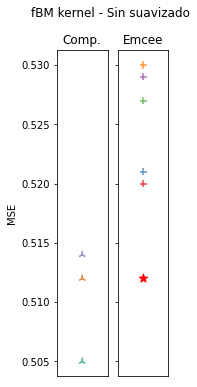
\includegraphics[width=0.31\textwidth]{img/results-new/reg_l2_fbm_none}\hfill
    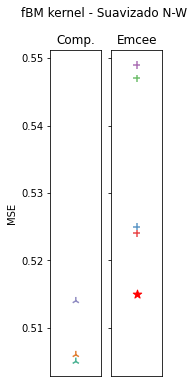
\includegraphics[width=0.3\textwidth]{img/results-new/reg_l2_fbm_nw}\hfill
    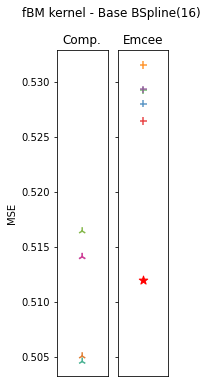
\includegraphics[width=0.31\textwidth]{img/results-new/reg_l2_fbm_basis}
    \caption{MSE de los mejores estimadores en cada caso bajo el modelo subyacente $L^2$ con kernel Browniano fraccional.}
  \end{figure}
\end{frame}

\begin{frame}{Resultados $\boldsymbol{L^2}$ kernel O-U}
  \begin{figure}
    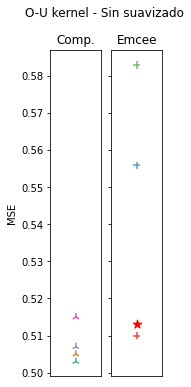
\includegraphics[width=0.3\textwidth]{img/results-new/reg_l2_ou_none}\hfill
    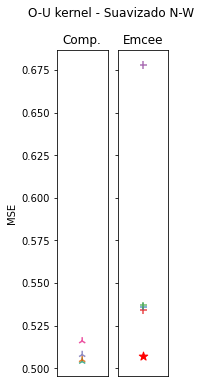
\includegraphics[width=0.31\textwidth]{img/results-new/reg_l2_ou_nw}\hfill
    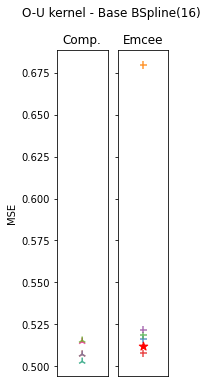
\includegraphics[width=0.31\textwidth]{img/results-new/reg_l2_ou_basis}
    \caption{MSE de los mejores estimadores en cada caso bajo el modelo subyacente $L^2$ con kernel de Ornstein-Uhlenbeck.}
  \end{figure}
\end{frame}

\begin{frame}{Resultados $\boldsymbol{L^2}$ kernel RBF}
  \begin{figure}
    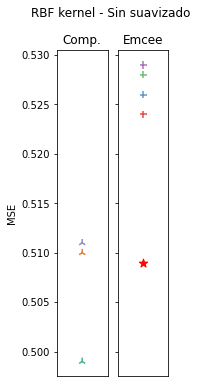
\includegraphics[width=0.3\textwidth]{img/results-new/reg_l2_rbf_none}\hfill
    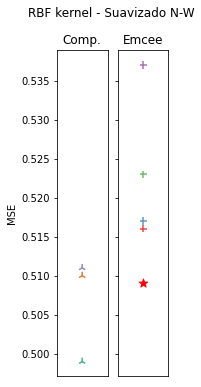
\includegraphics[width=0.3\textwidth]{img/results-new/reg_l2_rbf_nw}\hfill
    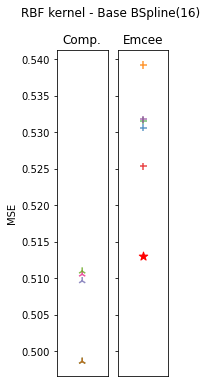
\includegraphics[width=0.31\textwidth]{img/results-new/reg_l2_rbf_basis}
    \caption{MSE de los mejores estimadores en cada caso bajo el modelo subyacente $L^2$ con kernel RBF.}
  \end{figure}
\end{frame}

%%%%%%%

\begin{frame}{Resultados Tecator}
  \begin{figure}
    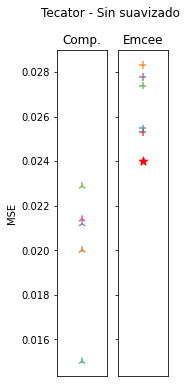
\includegraphics[width=0.3\textwidth]{img/results-new/reg_tecator_none}\hfill
    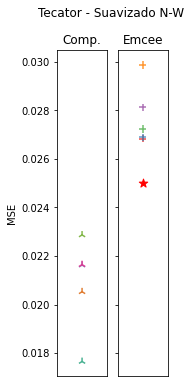
\includegraphics[width=0.3\textwidth]{img/results-new/reg_tecator_nw}\hfill
    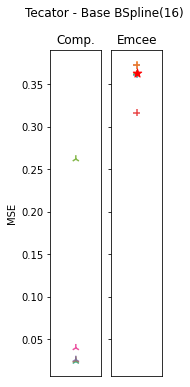
\includegraphics[width=0.3\textwidth]{img/results-new/reg_tecator_basis}
    \caption{MSE de los mejores estimadores en cada caso para el conjunto de datos Tecator.}
  \end{figure}
\end{frame}

\begin{frame}{Resultados Aemet}
  \begin{figure}
    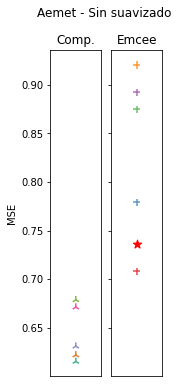
\includegraphics[width=0.28\textwidth]{img/results-new/reg_aemet_none}\hfill
    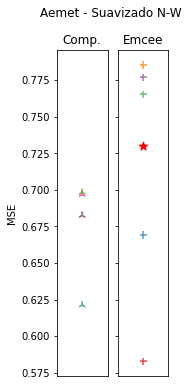
\includegraphics[width=0.3\textwidth]{img/results-new/reg_aemet_nw}\hfill
    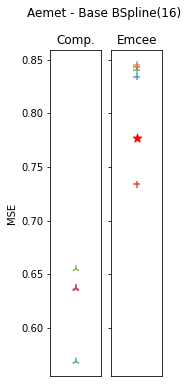
\includegraphics[width=0.3\textwidth]{img/results-new/reg_aemet_basis}
    \caption{MSE de los mejores estimadores en cada caso para el conjunto de datos Aemet.}
  \end{figure}
\end{frame}




\subsection{Regresión logística}

\begin{frame}{Resultados RKHS kernel fBM}
  \begin{figure}
    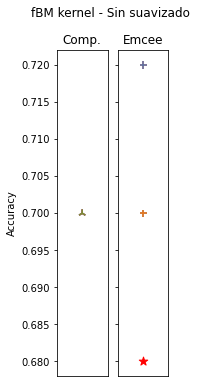
\includegraphics[width=0.295\textwidth]{img/results-new/clf_rkhs_fbm_none}\hfill
    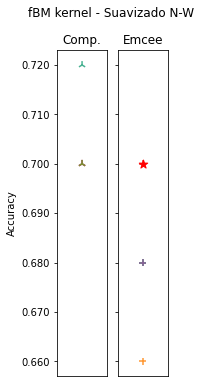
\includegraphics[width=0.3\textwidth]{img/results-new/clf_rkhs_fbm_nw}\hfill
    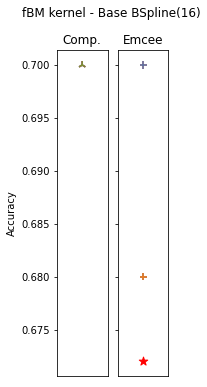
\includegraphics[width=0.31\textwidth]{img/results-new/clf_rkhs_fbm_basis}
    \caption{Accuracy de los mejores estimadores en cada caso bajo el modelo subyacente RKHS con kernel Browniano fraccional.}
  \end{figure}
\end{frame}

\begin{frame}{Resultados RKHS kernel O-U}
  \begin{figure}
    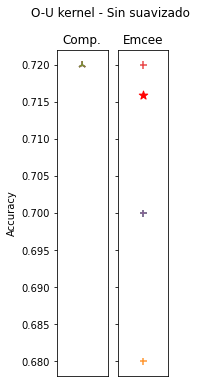
\includegraphics[width=0.295\textwidth]{img/results-new/clf_rkhs_ou_none}\hfill
    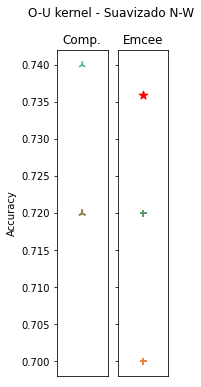
\includegraphics[width=0.3\textwidth]{img/results-new/clf_rkhs_ou_nw}\hfill
    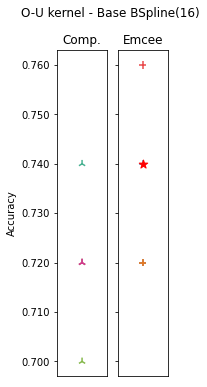
\includegraphics[width=0.31\textwidth]{img/results-new/clf_rkhs_ou_basis}
    \caption{Accuracy de los mejores estimadores en cada caso bajo el modelo subyacente RKHS con kernel de Ornstein-Uhlenbeck.}
  \end{figure}
\end{frame}

\begin{frame}{Resultados RKHS kernel RBF}
  \begin{figure}
    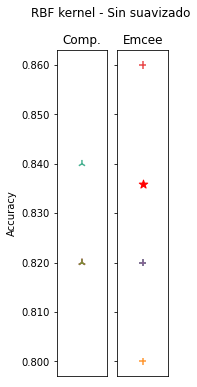
\includegraphics[width=0.3\textwidth]{img/results-new/clf_rkhs_rbf_none}\hfill
    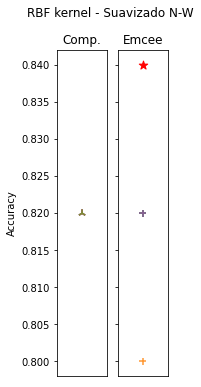
\includegraphics[width=0.305\textwidth]{img/results-new/clf_rkhs_rbf_nw}\hfill
    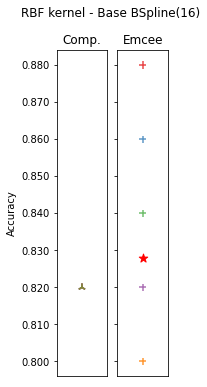
\includegraphics[width=0.315\textwidth]{img/results-new/clf_rkhs_rbf_basis}
    \caption{Accuracy de los mejores estimadores en cada caso bajo el modelo subyacente RKHS con kernel RBF.}
  \end{figure}
\end{frame}

%%%%%%

\begin{frame}{Resultados $\boldsymbol{L^2}$ kernel fBM}
  \begin{figure}
    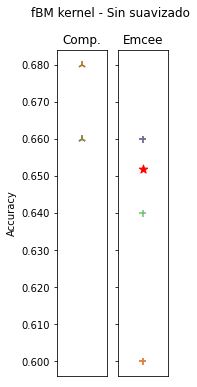
\includegraphics[width=0.3\textwidth]{img/results-new/clf_l2_fbm_none}\hfill
    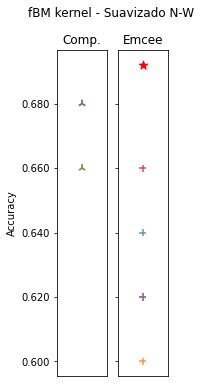
\includegraphics[width=0.3\textwidth]{img/results-new/clf_l2_fbm_nw}\hfill
    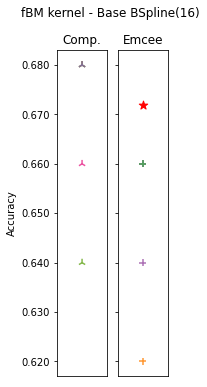
\includegraphics[width=0.31\textwidth]{img/results-new/clf_l2_fbm_basis}
    \caption{Accuracy de los mejores estimadores en cada caso bajo el modelo subyacente $L^2$ con kernel Browniano fraccional.}
  \end{figure}
\end{frame}

\begin{frame}{Resultados $\boldsymbol{L^2}$ kernel O-U}
  \begin{figure}
    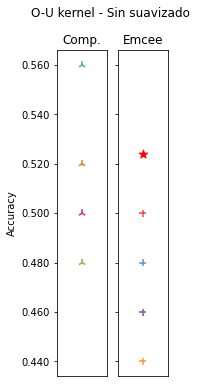
\includegraphics[width=0.3\textwidth]{img/results-new/clf_l2_ou_none}\hfill
    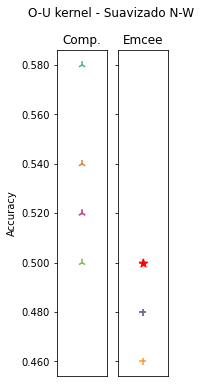
\includegraphics[width=0.3\textwidth]{img/results-new/clf_l2_ou_nw}\hfill
    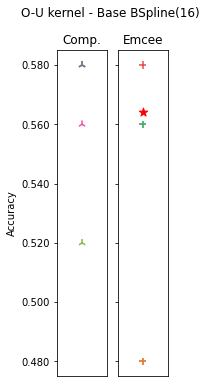
\includegraphics[width=0.31\textwidth]{img/results-new/clf_l2_ou_basis}
    \caption{Accuracy de los mejores estimadores en cada caso bajo el modelo subyacente $L^2$ con kernel de Ornstein-Uhlenbeck.}
  \end{figure}
\end{frame}

\begin{frame}{Resultados $\boldsymbol{L^2}$ kernel RBF}
  \begin{figure}
    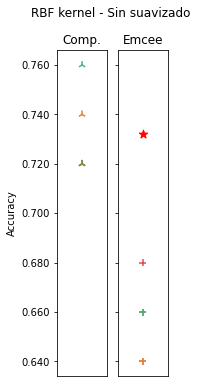
\includegraphics[width=0.3\textwidth]{img/results-new/clf_l2_rbf_none}\hfill
    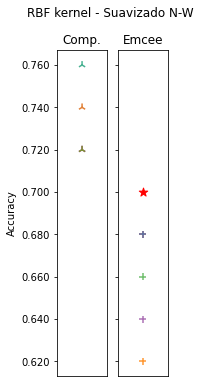
\includegraphics[width=0.305\textwidth]{img/results-new/clf_l2_rbf_nw}\hfill
    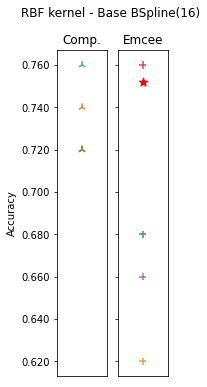
\includegraphics[width=0.31\textwidth]{img/results-new/clf_l2_rbf_basis}
    \caption{Accuracy de los mejores estimadores en cada caso bajo el modelo subyacente $L^2$ con kernel RBF.}
  \end{figure}
\end{frame}

%%%%%%%

\begin{frame}{Resultados Medflies}
  \begin{figure}
    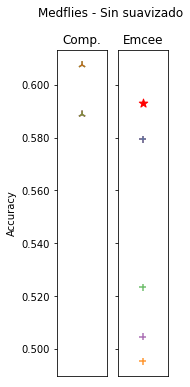
\includegraphics[width=0.3\textwidth]{img/results-new/clf_medflies_none}\hfill
    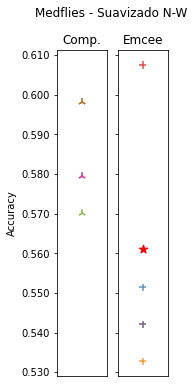
\includegraphics[width=0.305\textwidth]{img/results-new/clf_medflies_nw}\hfill
    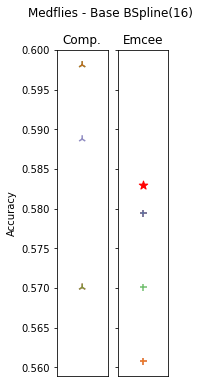
\includegraphics[width=0.315\textwidth]{img/results-new/clf_medflies_basis}
    \caption{Accuracy de los mejores estimadores en cada caso para el conjunto de datos Medflies.}
  \end{figure}
\end{frame}

\begin{frame}{Resultados Growth}
  \begin{figure}
    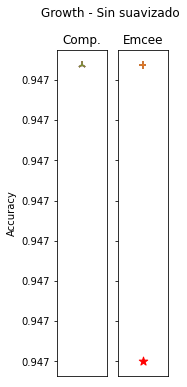
\includegraphics[width=0.3\textwidth]{img/results-new/clf_growth_none}\hfill
    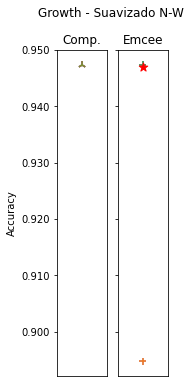
\includegraphics[width=0.3\textwidth]{img/results-new/clf_growth_nw}\hfill
    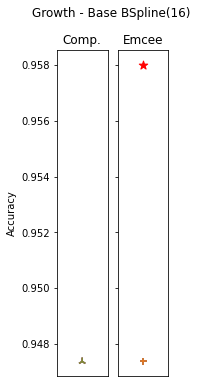
\includegraphics[width=0.31\textwidth]{img/results-new/clf_growth_basis}
    \caption{Accuracy de los mejores estimadores en cada caso para el conjunto de datos Growth.}
  \end{figure}
\end{frame}

\section{Referencias}
\begin{frame}{Bibliografía}

\printbibliography[heading=none]

\end{frame}

\end{document}
